\documentclass[a4paper,12pt]{article}
\usepackage{fancyhdr}
\usepackage{graphicx}
\usepackage[utf8]{inputenc}


\title{User Documentation}
\author{Group Project 3 - Group 2}
\date{April 08 2008}

\begin{document}
\maketitle
\newpage
\tableofcontents
\newpage



\section{Introduction and Overview}
\subsection{Introduction}
This material is provided to explain to an end user what the main features of the application are and how to use them, step by step.
An end user could be a seller, a buyer, or an estate agent.

\paragraph{}
The Napier Estate Agency Application is a Groovy/Grails website, we are not going to explain how to set-up the website,
we assume that this is not an end user task and that it will be handled by the IT department of your company.

\subsection{Main features}
The main feature of this application is the management of a property (registering a new property with its details, pictures, characteristics, and being able to edit it).
Because this is an important feature and will be one of the most commonly used, we are going to explain it fully in this document.

\section{For all users}
\subsection{Register and authenticate}

\section{Estate Agent}
\subsection{Manage a property}
\subsection{See properties status}
\subsection{Manage an appointment}

\section{Seller}
\subsection{Register a new property}
To register a new property, first you have to log-on to the website and click on "property management" on the left menu.

The property list will appear. Notice that you will see only the properties that you own (for a seller), or you manage (for an estate agent).
Now you can click on "New property" on the top action bar.
\begin{center}
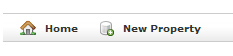
\includegraphics[scale=0.7]{pics/new_property.jpg}
\end{center}


A form will appear to allow you to enter all of the details. The first field (1) that you have to fill is the reference number of the property. Be careful, this number should be unique.

\paragraph{Visits time slots}

Then you have to fill the visit period field (2).
Just click on a date field and a mini calendar will appear, so you can easily select a date.
If you want to add another time slot for a visit just click on "Add line".

\paragraph{Property details}

The next fields (3) ask you usual information about your property, such as the address, the post code (must be a valid, well formatted UK postcode) and the number of bedrooms.

\paragraph{Owner and manager}

If you are logged on as a seller, you will be able to edit only the manager of your property. Just select it in the drop down menu.

\paragraph{Picture}

You shall upload some images of your property, several types of images are allowed, like jpeg, pngs or gifs.
Just click on the "Browse..." button (5) and an open file dialog will appear allowing you to select the image file on your computer.

\paragraph{Submit the property}
To submit your property, just click on the "Create" button (6). If there is some errors in your submission, the erroneous fields will be highlighted in red and you will be asked to correct your input.


\begin{center}
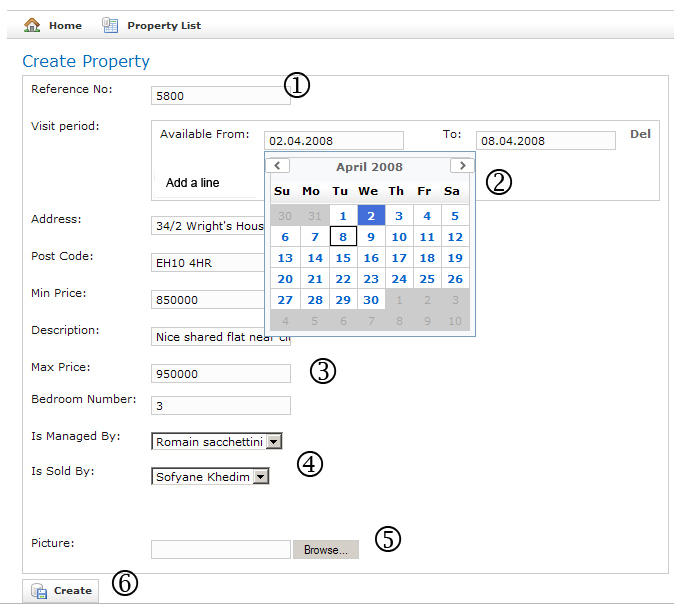
\includegraphics[scale=0.7]{pics/step_by_step.jpg}
\end{center}
\subsection{Edit your own properties details}

\section{Buyer}
\subsection{Browse and search properties}
\subsection{Set up a list of properties that you are interested in}


\end{document}